%\documentclass[a4paper,10pt]{article}
%\documentclass[a4paper,10pt,landscape]{article}
\documentclass[10pt]{article}
%\usepackage[landscape, a4paper, margin=20pt]{geometry}
\usepackage[a4paper, margin=20pt]{geometry}

%\usepackage[utf8]{inputenc} 
%\usepackage[square,sort,comma,numbers]{natbib}
%\usepackage[backend=biber,autocite=inline,style=authoryear]{biblatex}
\usepackage[backend=biber,autocite=inline]{biblatex}
\addbibresource{mybib21.bib}
%\usepackage{a4wide}
\usepackage{amsmath}
\usepackage{amssymb}
\usepackage{amsthm}
\usepackage{listings}
\usepackage{color}
\usepackage{enumerate}
%\usepackage{IEEEtrantools}
%\usepackage[redeflists]{IEEEtrantools}
\usepackage{verbatim}
\usepackage{graphicx}
\usepackage{subcaption}
\usepackage[section]{placeins} %no trans-sectional figures!
\usepackage{wrapfig, framed, caption}
\usepackage{slashbox}

\usepackage{booktabs} % For \toprule, \midrule and \bottomrule
\usepackage{siunitx} % Formats the units and values
\usepackage{pgfplotstable} % Generates table from .csv
% Setup siunitx:
\sisetup{
  round-mode          = places, % Rounds numbers
  round-precision     = 2, % to 2 places
}

\usepackage{hyperref}
\hypersetup{linktocpage,
            linktoc=all,
            %colorlinks=true,
            %linkcolor=blue,
            }

\usepackage{lipsum}
%\usepackage[onehalfspace]{setspace}
\usepackage{setspace}

% Basic data
\newcommand{\N}{\mathbb{N}}
\newcommand{\C}{\mathbb{C}}
\newcommand{\ASSIGNMENT}{2}
\newcommand{\B}{\{-1,1\}}
\newcommand{\E}{\mathbf{E}}
\newcommand{\F}{\mathbb{F}}
\newcommand{\Inf}{\textbf{Inf}}
\newcommand{\I}{\mathbf{I}}
\newcommand{\NS}{\textbf{NS}}
\newcommand{\R}{\mathbb{R}}
\newcommand{\Z}{\mathbb{Z}}
\newcommand{\aufgabe}[1]{\item{\bf #1}}
\newcommand{\bvec}[1]{\mathbf{#1}}
\newcommand{\bv}[1]{\mathbf{#1}}
\newcommand{\ceil}[1]{\lceil{#1}\rceil}
\newcommand{\floor}[1]{\lfloor{#1}\rfloor}
\newcommand{\gt}{>}
\newcommand{\half}[1]{\frac{#1}{2}}
\newcommand{\lt}{<}
\newcommand{\tuple}[1]{\langle #1 \rangle}

\newcommand{\suftab}{\text{suftab}}

\setlength{\parskip}{1.0em}
\setlength{\parindent}{1em}


\lstset{
%basicstyle=\footnotesize,
%basicstyle=\ttfamily\footnotesize,
%basicstyle=\ttfamily\small,
%basicstyle=\ttfamily\scriptsize,
frame=single,
%numbers=none,
%numbersep=5pt,
numberstyle=\tiny,
showspaces=false,
showstringspaces=false,
tabsize=2,
breaklines=true,
%escapeinside={#*}{*#},
escapeinside={$}{$},
%escapeinside={*\&}{\&*},% if you want to add LaTeX within your code
%mathescape=true,
%language=C++
}

\theoremstyle{definition}
\newtheorem{mydef}{Definition}[section]

\theoremstyle{remark}
\newtheorem{remark}{Remark}

\theoremstyle{plain}
\newtheorem{thm}{Theorem}[section]
%\newtheorem{thm}{Theorem}[mydef]
\newtheorem{lemma}{Lemma}[section]
%\newtheorem{lemma}{Lemma}[mydef]

\begin{document}
\renewcommand{\thesubsection}{\thesection.\alph{subsection}}\renewcommand{\thesubsection}{\thesection.\alph{subsection}}


% Document title
\begin{titlepage}
    \title{Notes about Function Prediction}
    \author{Yiftach Kolb}
    %\author{\_\_\_\_\_\_\_\_\_\_\_\_\_\_\_\_\_\_}
    \date{\today}
\end{titlepage}

\maketitle

\section{RWR Methods}

\subsection{go by rows or columns?}
we have a graph $G(V,E)$ and we associate with it a transition
matrix $T$ of size $n \times n$. Now one thing to be carefule about is whether the rows
or the columns of $T$ are normalized.

If the rows are normalized, then $T_{i,j}$ represents the transition
probability from $i$ to $j$. If $p = (p_1, \dots p_n)$ is a row
vector representing then $p \cdot T$ is the next probability in the 
process.

But for me at least, I prefer to use the standard matrix
multiplication so we can transpose $T$ and $p$:  $A = T^{t}, u =
p^{t}$, so now $A$ is column normalized and $u$ is a column vector
and $A \cdot u$ is the next distribution of the process.

Anyway from now on lets assume by convention that a transition
matrix is column-normalized and vectors are column vectors by
default.


\subsection{RWR by matrix representation}
So here we have a transition matrix $T$ derived from the graph $G$.
Let $q$ a fixed
distribution on the vertices  $\{1 \dots n\}$ (column vector).
Fix $\alpha \in [0,1]$, representating the restart probability.

We can now define the RWR as the sequence of distributions $p_i$ defined
by:
\begin{itemize}
\label{def:RWR}
\item{} $p_0 := q$ (doesn't really matter what $p_0 \neq 0$ we
choose, they all converge to the same, greatest eigenvector)
\item{} $p_{k+1} := (1 - \alpha) T \cdot p_k + \alpha q$
\subitem{} 
If we let $Q$ be the matrix with all
columns $q$, $Q := (q | \dots | q)$ then we may rewrite the
transition step as:

$p_{k+1} = 
[(1-\alpha) T + \alpha Q] \cdot p_k$
\end{itemize}

This process converges to a stationary distribution $p = \lim p_k$.
So we get 
\begin{equation}
p = (1 - \alpha) T \cdot p + \alpha q
\end{equation}

We can rewite this:
\begin{equation}
(I - (1 - \alpha)T) \cdot p = \alpha q. 
\end{equation}

The matrix $I - (1 - \alpha)T$ is invertible, so we can solve $p$
from $q$ and we get:

\begin{equation}
\label{def:RWRp}
p = \alpha (I - (1 - \alpha)T)^{-1} q := K \cdot q 
\end{equation}

This is in my opinion a very important result.
It means we choose a restart distibution and from it we get the
stationary distribution of the corresponding RWR process.

Let say that we choose $q = (1,0,\dots 0)$ Then $p = K \cdot q$ will
be the stationary distribution for the RWR with restart to node $1$
(with probability $\alpha$. This is what propagating from node $1$
means.

If we choose $q = (1/n \dots 1/n)$ then the corrsponding stationary
$p = Kq$ is the pageRank distribution. so $p[i]$ (its i'th
component) would be the pagerank of node $i$.

The matrix $K$ from \ref{def:RWRp} is closely related to the graph
Laplacian and in fact $K^{-1}$ and this is why in the Laplacian we
are interested in the smallest eigentvectors whereas in the 
transition matrices ($K$ is also a transition matrice) we are
interested in the largest eigenvalues. More on that in the next
subsection.

\subsection{predicting multiple functions per protein}
If we have labels $f$ and $g$, it is easy to answer using RWR if an 
unlabled vertex $v$ is more $f$ or more $g$\textemdash whichever
scores higher for $v$ is the likelier function. But it could be that
$v$ actually has both functions. I have to imagine that in actuality
function annotations have overlap or inclusion relations in many
cases.

The scores as we will see below, are computed independently for each
label. So it makes sense for  a threshold 
to be set, and if $f$ scores for $v$ above
set threshold than $v$ has label $f$ (not necessarily exclusive).

\subsection{Relation to the Laplacian matriced and spectral
clustering}

This is an excerpt from the spectral clustering part which had been
left out of my bachelor's thesis. I include it here because
there is a very strong connection between graph laplacians and
the diffusion matrix. We talked about how in the Laplacian
we look for the smallest eigenvalues instead of the largest and the
reason for that is very simple- the Laplacian's eigenvalues
correspond to the diffusion matrix's (and to the orifinal transition
matrix of $G$) in inverse order.

\begin{mydef}
\label{def:Laplacian}
Let $G$ be a bidirectional graph with adjacency matrix $A$ and diagonal degree
matrix $D$.
Then the following matrices are its \textbf{graph Laplacian}, and its
\textbf{symmetric\textemdash
, row\textendash normalized\textemdash and column\textendash normalized\textemdash Laplacians}:  

\begin{equation}
\begin{aligned}
L & = D - A \\
L_s & = D^{-1/2}LD^{-1/2} = I - D^{-1/2}AD^{-1/2} \\
L_r & = D^{-1}L = I - D^{-1}A \\
L_c & = LD^{-1} = I - AD^{-1}
\end{aligned}
\end{equation}
\end{mydef}

Consider the connected graph $G$ and its adjacency matrix $A$. We create the transition
matrix by normalizing it: $T = AD^-1$, and finally we choose a restart parameter
$\alpha$ and create the diffusion matrix $K = \alpha[I - (1 -
\alpha) T]^{-1}$. 
$K$ and $T$ have the same
eigenvectors and the orders of their corresponding eigenvalues are the same. The
eigenvalues are all real and therefore the eigenvectors are real as well. And
the eigenvalues of $K$ are all non-negative.

The matrix $K^{-1} = \alpha^{-1} [I - (1- \alpha) T]$ is closely related to the
symmetric Laplacian $L_s$ and thecolumn-normalized Laplacian $L_c$. The added parameter $0 \lt \alpha \lt 1$
neither changes the eigenvectors, nor the order of the corresponding eigenvalues.

The smallest eigenvalue ,$0$ of $L$ and $L_s$
corresponds to the largest eigenvalue $1$ of and $T$ and its eigenvector is
(can be chosen as) all positive. 
Any other eigenvector of $L$ (which corresponds to an eigenvector of $T$) must
contain both positive and negative components (Perron-Froebenius).




\subsection{Using RWR to predict a function of an unlabled protein}

\begin{mydef}
\label{partialmultilabeling}
Let $V = \{1 \dots n\}$ be the vertex set,
let $\mathcal{L} = \{f_1, \dots f_p\}$ a set of labels.

A \textbf{partial (multi) labeling} of $V$ is a function
$\delta : V \times \mathcal{L} \to \{0,1\}$
$v \in V$ has label $f \in \mathcal{L}$ iff $\delta(v,f)=1$.
This definition allows for vertex to have multiple labels.
\end{mydef}

We saw in \ref{def:RWRp} that for each restart distribution there is
a corresponding stationary distribution of the RWR. The idea of
propagation is to set for each $v$ a restart distribution $q_v$ (as
a column vector), which then yields a stationary distribution $p_v =
K \cdot q_v$ that we associate with vertex $v$.

We can use matrix notation: let $QR = (q_1| \dots | q_n)$ be the
matrix of restart distribution, such that column $v$ of $QR$ is
$q_v$. Then let $PR = K \cdot QR = (p_1| \dots |p_n)$ 
(so the $p_i$'s are \textbf{column vectors}), the
corresponding matrix of stationary distributions, so that the first
column is $p_1 = K \cdot q_1$ the stationary distribution we
associate with vertex $1$ etc.

The question is how to choose the right restart distribution for
each $v$.
In my bachelor thesis, I picked $q_v = e_v$ where $e_v$ is that
standard indicator vector (so it has $1$ on coordinate $v$ and is
$0$ otherwise). This means in the RWR process for $v$ we restart
from $v$ with probability $\alpha$.
In the article of Zhang et. al, they defined a different $q_v$ which
is a distribution on all the vertices based on some similarity
calculations they do which takes into account both graph topology
(shared vs. unique neighbors) as well as protein domains comonality.
They also didn't use the PPI graph itself for the propagation,
rather they defined a correlation matrice based on that graph.

Now that we have for each vertex $v$ an associated stationary
distribution $p_v$, we need a way to claculate the label score for
each label for each protein, and it is straitforward:

\begin{mydef}
\label{def:scorefunction}
The score function $s$ is the function
$s : V \times \mathcal{L} \to [0,1]$ defined by
$s(v,f) = \sum_{i \in V}p_v[i] \cdot \delta(i,f)$
\end{mydef}

So $s(v,f)$ is the score of label $f$ for vertex $v$, which in my
bachelor's thesis I called the 'volume' but I now use the score term
which I like more and is used by Zhang et. al.

In my thesis, for methods 1 and 2 I took 
$g_v = \text{argmax}\{s(v,f) | f \in \mathcal(f)\}$ as the predicted
function of $v$. In Zhang et. al. they pick the $K$ largest argument as the
predicted function set for $v$.

\section{a note about the difference between scoring and ranking}
Using the same notation as above, if we set the restart distribution
as the uniform one, $q = (1/n, \dots , 1/n)$, which means in our
RWR we make every node equally likely to be restarted from.
We obtain the corresponding stationary distribution $p = K \cdot q$
of this walk.

Now in PageRank, the vertices are then ranked according to their 
components in $p$. So the highest ranked vertex is
$v = \text{argmax}\{p[i] | i \in V \}$.
$p[i]$ is the frequency in which $i$ is visited in the RWR, so $v$
is the most frequently visited vertex.
In the case of 
context search we would say that $v$ is the top result and 

In my bachelor thesis I used this principle for method 5.
Basically suppose we have two disjoint subsets 
$A, B \subset V$. Now we set $q_a$ to be the uniform distribution
over members of $A$ (and $0$ outside $A$), and similarly with $q_b$
for $B$.

we get two different RWR processes dependent whether we pick $q_a$
or $q_b$ for the restart, so we also get the two corresponding 
stationary distributions of these RWRs:
$p_a = K \cdot q_a$ and $p_b = K \cdot q_b$.

Now given vertex $i \in V - (A \cup B)$, we can compare
is $i$ visited more frequently when we restart from $q_a$
(a random member of $A$) or from $B$?
$p_a[i] \square ? p_b[i]$
And according decide if $i$ more likely belong to $A$ or to $B$.


\begin{figure}[htb!]
\begin{framed}
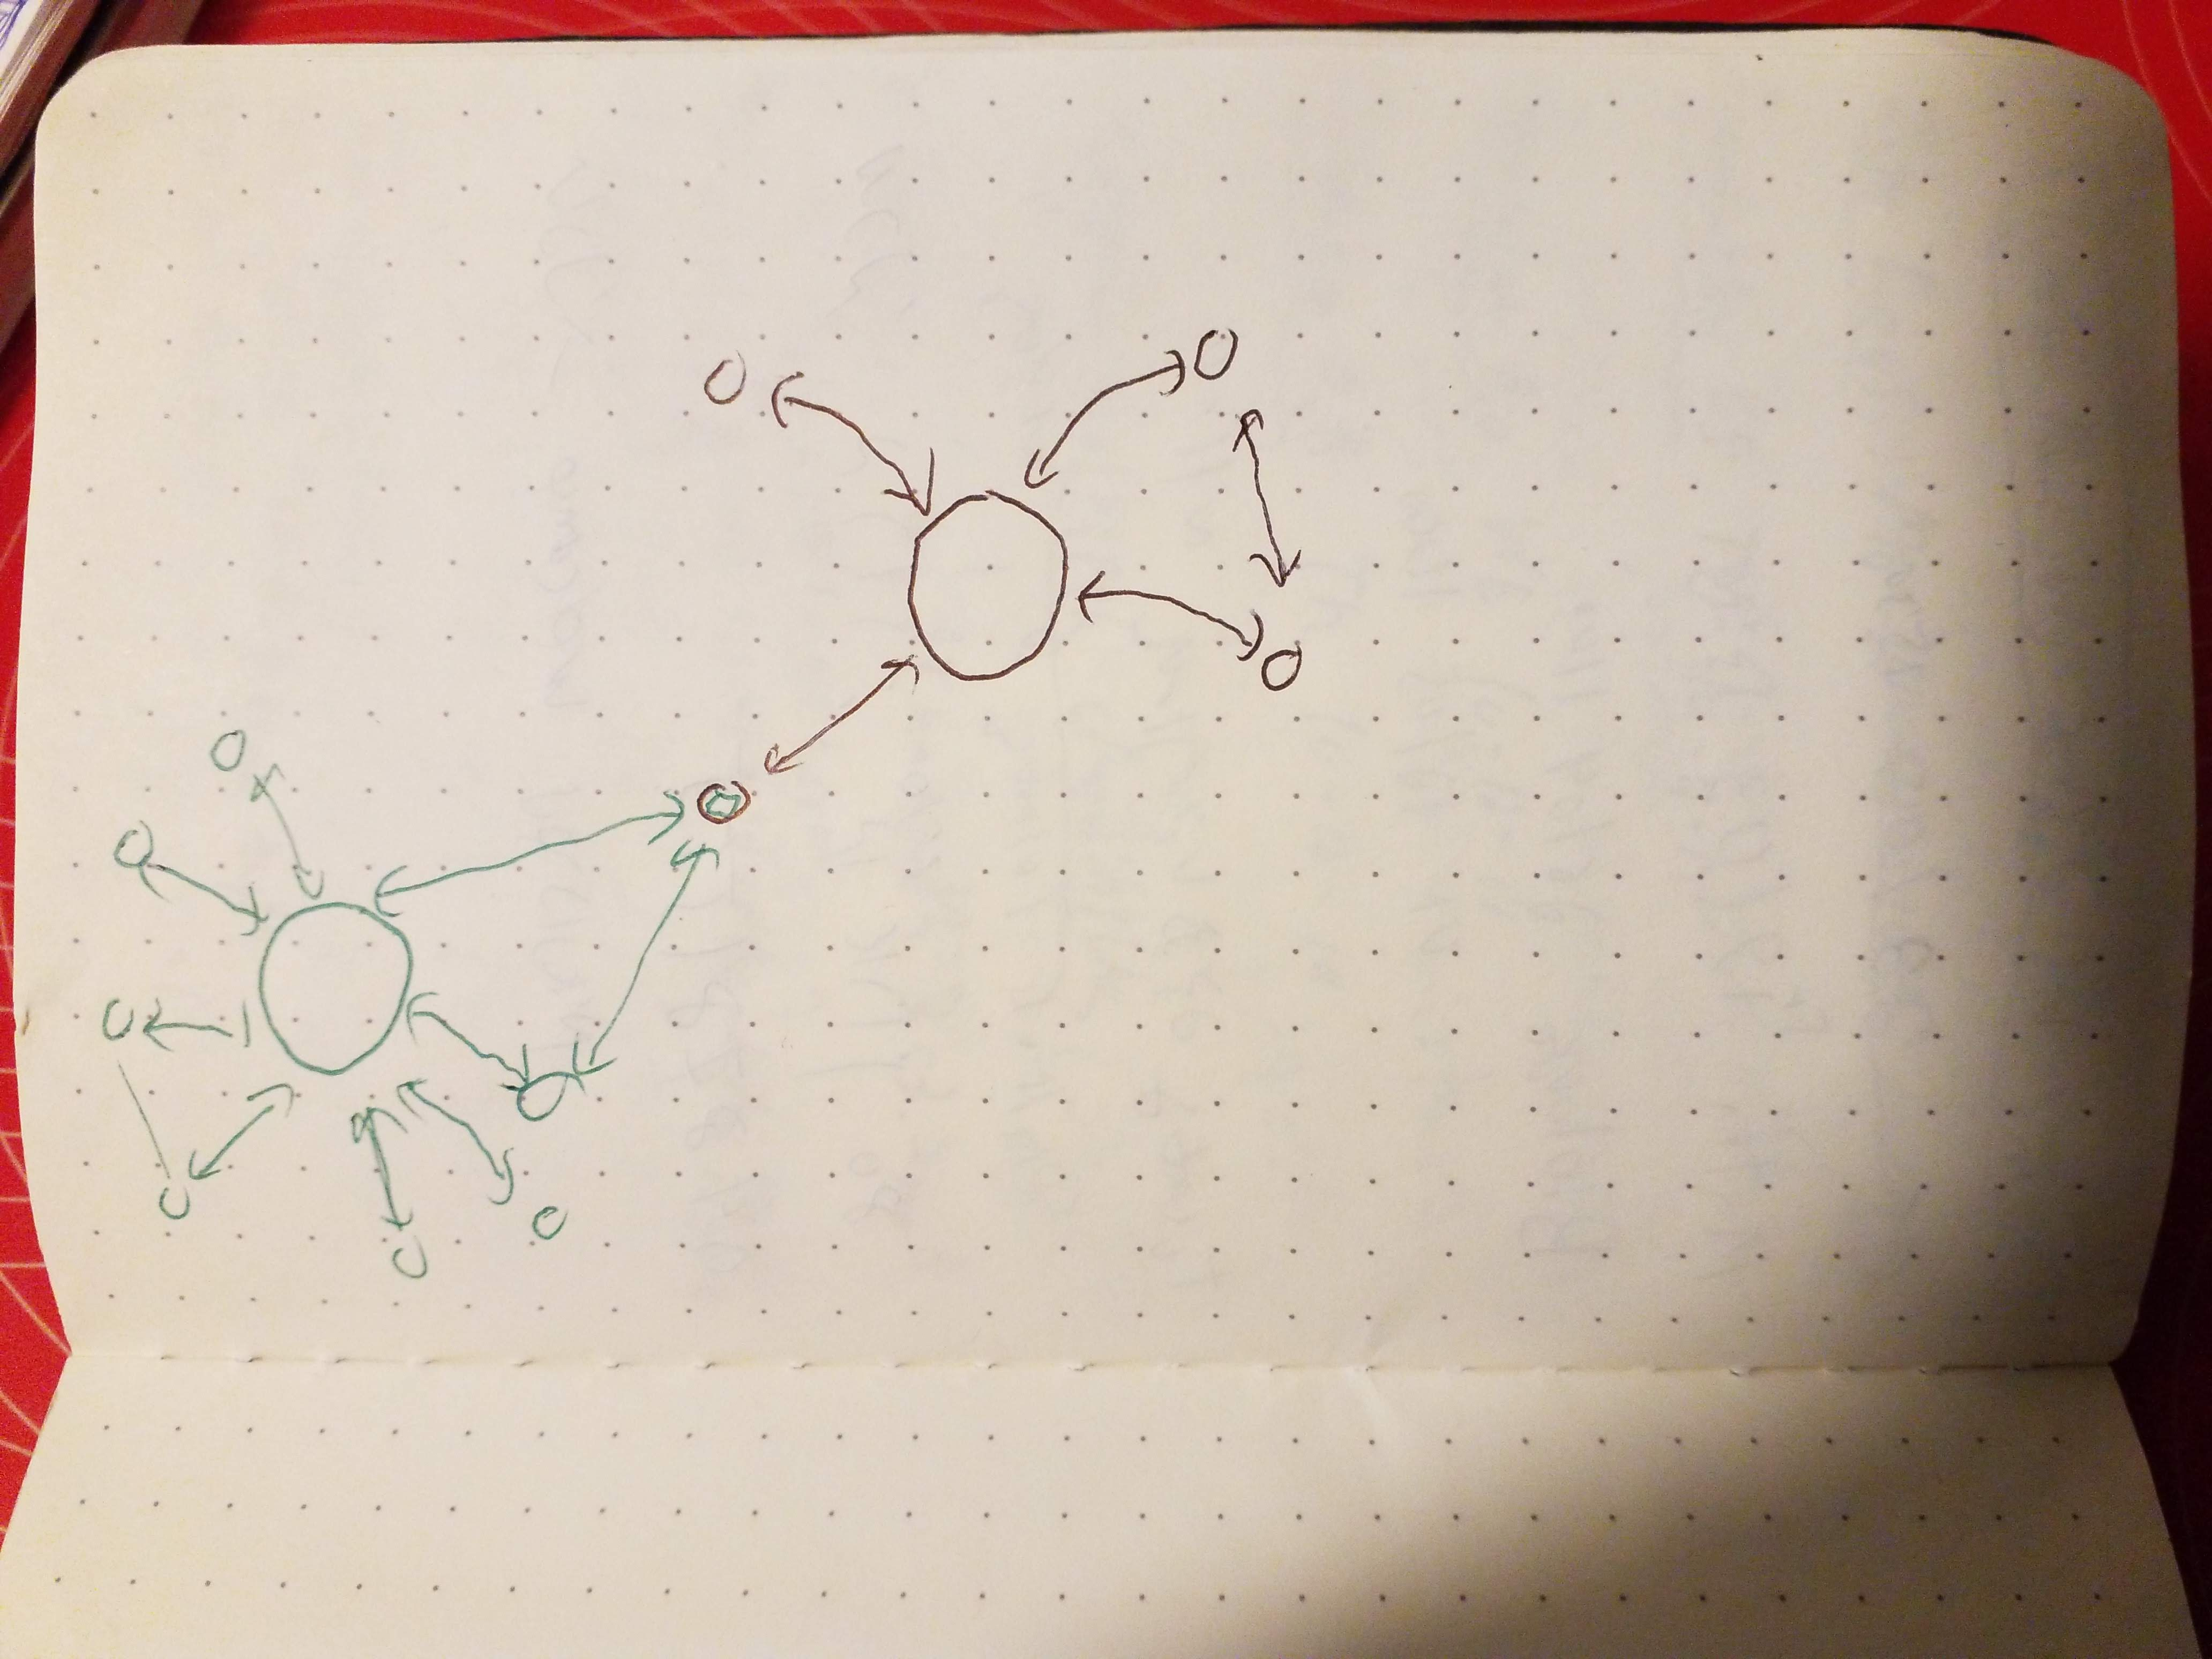
\includegraphics[width=\textwidth]{./images/plot00.jpg}
\caption{Example where ranking fails but scoring works}
\label{fig:rankvsscore}
\end{framed}
\end{figure}

In figure~\ref{fig:rankvsscore} I try to demonstrate this scoring vs.
ranking idea. We want to predict the function of the vertex in the
middle, is it black or green? All the other vertices are known to be
black or green.

If we do a random walk with uniform restart to a any green node, and
a random walk with restart to any black node, then compare the
frequencies in which the node in question is visited in each
process,
then we would probably find out that it is visited more frequently 
when we restart to the black group, simply because the black module
is smaller than the green module so it is more likely to get out of
it and visit the node in the middle. 

If we do a restart to the green group, since this module is much
larger we will probably visit the node in question less frequently
even though it it is more connected to the green module than to the
black module.

However, if we try to predict to which module the node in the middle

belongs to, by doing a RWR with restart to the node itself,
then clearly in this process we visit a green node more frequently
than a black node. Therefore the score of the greens (which is the
sum of the frequencies of all the green nodes in this RWR) will be
higher.

\section{Summary of Methods used in different articles}
\subsection{NPF (Zhang et al)}
\begin{framed}
\subsubsection*{TLDR}
They "stole" my score function.

They use information for domain similarity and complex commonalities
to define a restart distribution for each protein. So instead of
restarting to the protein itself, they restart to proteins that are
somehow similar to it.

They create the "co-neighbor" network out of the adjacency matrix
and that is the matrix they propagate with (with restart).
So in my recipe I try for example to borrow core normalization
from Gal.

The resulting propagation matrix which they call $PN$ is used to
extract "modules" but there is something strange with the math
there. They use what they call neighbor fitness to thin out the
neighbors of the node of interest. Come up with candidate functions
out of it, and use score to rank these candidates.
\end{framed}

This method takes the original PPI network (lets call it $G$) and
constructs a "Co-neiboughr network", which is a weighted graph based
on neighbor correlations. This is the network that the RWR is done
in, not the original PPI network.

For the restart distributions, they combine two distributions.
One uses 'protein-complex' the other uses a 'protein-domain matrix'.
To every protein they calculate its own restart distribution, to be
clear, it measns when RWR is done to predict functions to said
proteins, the restart is not only to the protein itself but any
protein can be restarted from with probability that is proportional
to its combined domain/complex correlations to the said protein.

Then they use RWR with the
restart distributions calculated to that protein. So every protein
has its own stationary distribution out of this process and the
combined result is a matrix (the PN or propagation network).

For the function prediction, they first use something they call
neighbor fitness to screen out neighbors of a protein from the PN
network. Then the predict the $K$ top scoring labels as the
functions of the protein. $K$ is the number of labels 
of the most functionally 
(annotated) vertex to the one they try to predict.
They define $PN(v,u)$ as the function similarity between $u$ and
$v$.
$\dots$



\subsection{Jaakola}

His solution considers a fixed time scaled random walk without
restart. So his transition matrix is $T^t$, where $T$ is the
transition matrix of the network. But I think this solution can be
applied just as well for RWR by replacing that matrix with $K$, the
diffusion matrix. In his article he uses normalized rows instead of
my prefered normalized column and right multiplication.  I will
try to stay consisten and use only column normalizations.

$P_{t | 0}(k | i):= p^t_{ik} = [T^t]_{k,i}$ 
is the probability to end at $k$, given that we
started from $i$, after exactly $t$ steps without restart.

We now want to evaluate the probability that the 
Markov process started from $i$ given that it ended
in $k$, and call it: $P_{0 | t}(i | k)$. 
Jaakola assumes that every vertex is equally likely to be started
from $p_{\text{start}}(k) = 1/n$. Using this and the transitions,
we can calculate the probability for to end at $k$ for each $k$, 
which is $p_{\text{end}}(k) = \sum_i \frac{p^t_{ik}}{n}$.
Then 
we can use Bayes' Formula
to calculate this probability:
$P_{0 | t}(i | k) = 
\frac{P_{t | 0}(k | i) p_{\text{start}}(i)}{p_{\text{end}}(k)} 
= \frac{p^t_{ik}}{\sum_j p^t_{jk}}
$

Now we come to the labeling. We assume the the first
$l$ vertices are labeled with labels $y_i, i = 1 \dots l$.
The labels come from the set $y_i \in \{1 \dots C\}$.

We assume that every node has a distribution of the labels:
$P(y | i)$, which is unknown for labels $l+1 \dots n$ and we 
need to solve or estimate it. For the first $l$ node this distribution is
concentrated on the given label so $P(y=y_i | i) = 1$.
This $P(y | k)$, to my understanding is used as the prior
probability for the labeling.

Now we define the posterior distribution that vertex $k$ has
label 
$y$: 
$P_p(y | k) = \sum_i P(y | i)P_{0 | t}(i | k)$
So here the thought of is that, given that the
walk ended in $k$, we sum over all the possibilities of the process
originated in $i$ and that $i$ was labeled $y$.

Finally the predicted label $y$ for $k$ is the label $y=c$ which
maximizes that posterior probability.

To my understanding we can simply plug $p^t_ik = K_{k,i}$ in these
formulas to make it applicaple for a RWR instead of a fixed time
scale $t$ without restart.

In the Jaakola paper, two methods are used for estimation of
$P(y | k)$. The first is an EM algorithm.

The second is linear programming. For the linear program, they
provide the solution which is:


$P(y=c_i | i) = $
$\begin{cases}
1 \text{ if } c_i = \text{argmax}_c\frac{1}{N_c}
\sum_{k\leq l, y_k=c}P_{0|t}(i|k)\\
0 \text{ otherwise}
\end{cases}
$
Where $N_c$ is the number of vertices labeled with $c$ among 
the known labled vertices $1 \dots l$.

So for $P(y|k)$ the suggested solution is to look the probability
that the process started from a known 'red' node (vs a 'green' node,
etc.), given that it ende in node $k$. $P(y|k)$ is then going to be
concentrated on the color that maximized this probability.

Then for the posterior we use these priors for the labels of all
vertices not just the unknow ones, and we find the label that
maximizes that posterior: so lets say red maximized the probability
that we started at any initial node and it was red, (vs green
etc.). 

This solution is 'wholistic' in the sense that it considers the
graph as a whole and gives every node an equal chance to be the
initial node. I think there might be here as well a problem of
scale, so large groups have more influence because we are more
likely starting from them.


























\begin{comment}
He degree-normalized the rows, so 
$p_{i,k} = W_{i,k}/(\sum_j W_{ij})$ and in his notations
the transition matrix is $A = (p_{i,k})_{i,k}$.
Then define $P_{t | 0}(k | i) = [A^t]_{i,k}$ the 
conditional probability to end in $k$ if we start in $i$ after
exactly $t$ steps.
We assume the starting probability is uniform $P(i) = 1/n$, meaning
we don't know where we started and every node is equally likely.

We now want to evaluate the probability that the 
Markov process started from $i$ given that it ended
in $k$, and call it: $P_{0 | t}(i | k)$.

Let $F = \{1 \dots C\}$ be the set of labels. For $y \in F$
the posterior probability of the label for node $k$ is:
$P_{Pt}(y | k) = \sum_i P(y | k)P_{0 | t}(i | k)$
Finally the predicted function is the one that maximizes this
probability: $c_k = \text{argmax}_y P_{Pt}(y|k)$.

Note that using our assumptions and Bayes law we can calculate $P_{0
| t|}(i | k) = P_{t | 0}(k | i)P(i) / \sum_i P_{t | 0}(k | i)$

So the parameters we need to solve/estimate are $P(y | k)$.

Jaakola suggests two methods to estimate $P_{Pt}(y | k)$.
The first is to use the EM algorithm. I think we have mentioned all
the components needed for the E and M step but admittedly I am not
familiar with the EM algorithm, form the descryption it works like
something we called posterior decoding if I am not mistaken.

A second solution uses something Jaakola calls margin based
estimation. It gives a different estimation, it is not equivalent to
the first method. The margin of the classifier
on node $k$ and class $d$ is defined
$\gamma_{kd} = P_{Pt}(y = y_k | k) - P_{Pt}(y=d | k)$,
where $y_k \in F$ is the class predicted by the classifier
for node $k$.

For a correct classification the margin must satisfy:
$\forall k,d \gamma_{kd} \geq 0$ and for the correct class $y_k$ 
it must be $\gamma_{k y_k} = 0$.

Let $C$ be the number of different classes and $N_{C(k)}$ the number
of nodes labeled the same label as node $k$ (that is of the known
nodes, it appears that he doesn't update this count on the fly). 
Let $L$ be the number of labeled nodes we start with (so nodes 
$1 \dots L$ start with a known label).
Then he obtains a linear which well, one aspect of which I couldn't
understand. But fortunately he gives the solution and it is:
$P(y=c_i | i) = 1$, if $c_i =  \text{argmax}_C 
\frac{1}{N_C} \sum_{k\leq L : y_k = c} P_{0 | t}(i | k)$ and $0$
otherwise.

So just to be clear the $y_k$ for $k = 1 \dots L$ are the known
labeled nodes (the first $L$ proteins).

If I try to sum up what Jaakola proposes: he estimates for every
node the distributions of the labels over that node, $P(y | i)$. So
$\sum_y P(y | i) = 1$. He finds an estimation for these distribution
and you would think that was it and let the $y$ that maximized $P(y
| i)$ be the label of $i$. But that's not enough for Jaakola,
because according to his model We start a walk from an unknown node
and $P_{Pst}(y | k)$ is the probability that we end in $k$ and we
started from $1$, ended in $k$ ,and $1$ was labeled $y$, or we
started from $2$ ended in $k$, and $2$ was labeled $y$ or \dots.

Interestingly his solution for $P(y | i)$ is track backs to the
original $L$ labeled nodes.
Recall that $P_{0 | t}(i | k)$ is the probability that we started in
$i$ given that we ended in $k$. So for each label $y=c$, we check
the average of $\{P_{0 | t}(i | k) : y_k = c\}$. The $c$ which gives
the highest average of all labels is the one we concentrate $P(y|i)
= 1$ if $y=c$, or $0$ otherwise.

Usually in propagation we deal with probabilities where we assume we
(re)start from a certain subset, and check what is the probability
to land in the node of interested assuming a certain starting
position.

And I suppose in statistics lingo
that $P(y|i)$ is our prior estimation and finally we use it to
calculate the posterior.

%$\max_{P(y|i), \gamma_{kd}} \frac{1}{C(C-1)} 
%\sum_{k=1}^{L} \sum_{d=1}^{C} \frac{\gamma_{kd}}{N_{C(k)}}$
%subject to:
%$P_{Pt}(y=y_k$

\end{comment}

% references
\section{Reference}
\nocite{slides_from_lecture}
\nocite{cowen2017network}
\nocite{vandin2012discovery}
\nocite{leiserson2015pan}
\nocite{newman2006modularity}
\nocite{serre2010matrices}
\nocite{choobdar2019assessment}
\nocite{barel2020netcore}
\nocite{szummer2002partially}
\nocite{vanunu2010associating}
\nocite{zhao2020npf}




\printbibliography

\listoffigures
\listoftables



\end{document}
